
\documentclass[twocolumn, amsmath]{revtex4}

\usepackage{graphicx}



\begin{document}


\title{PHYS 605 Lab \#8} 

\author{Morgan A. Daly}
\author{Evin O'Shea}
\date{\today} 


\maketitle


\section{Introduction and Theory}
\subsection{Purpose}

This lab used the concepts of digital logic to solve a ``real world" problem.

First, a circuit involving NAND gates was constructed based on a schematic diagram provided. The goal was to demonstrate the behavior of NAND gates, and to generate a truth table for the circuit.

The next objective was to build a circuit that drives LED's so that they light in an alternating pattern (like lights on a school bus) using a 555 timer and NAND gates.


\subsection{Background / Theory}

Digital circuits consist of different high square pulses that can be categorized as one of two states: high or low, 1 or 0. This type of circuitry is often used in technology because it can send encoded data without error. The error is reduced, because a low and high pulse can be easily distinguished even with noise in the signal. This means that the data is only limited by the number of pulses sent.

In the lab, the group used LED's to get a visual feedback on the output of the circuits. 
LED's require a minimum voltage across them to light up. This works well in digital circuits, as the high voltage is over the diode voltage and the low is below it. This means that the LED on is a high coming through and the LED off is as low coming through.

The NAND gate performs the logical operator of ``not and". The truth table for this gate is shown below:

\begin{center}
	\begin{ruledtabular}
    \begin{tabular}{ l l l}
	IN$_1$ & IN$_2$ & OUT\\ \colrule
	0 & 0 & 1 \\
	0 & 1 & 1 \\
	1 & 0 & 1 \\
	1 & 1 & 0  \\
\end{tabular}
    \end{ruledtabular}
\end{center}

However, when the inputs are connected and therefore the same value, there are only two cases. This truth table is shown below:

\begin{center}
	\begin{ruledtabular}
    \begin{tabular}{ l l}
	IN & OUT\\ \colrule
	0 & 1 \\
	1 & 0 \\
\end{tabular}
    \end{ruledtabular}
\end{center}

When the inputs are tied together, the NAND gate inverts the signal. 

The circuit used in the lab is shown in figure (1). Three NAND gates configured in this way have their own truth table. The inputs to the first two NAND gates will be inverted, due to each terminal receiving the same input. The final NAND gate will have the standard ``not and" behavior shown in the first truth table. The truth table shown below is the equivalent truth table for the three gates:

\begin{center}
	\begin{ruledtabular}
    \begin{tabular}{ l l l}
	IN$_1$ & IN$_2$ & OUT\\ \colrule
	1 & 1 & 1 \\
	1 & 0 & 1 \\
	0 & 1 & 1 \\
	0 & 0 & 0  \\
\end{tabular}
    \end{ruledtabular}
\end{center}

This truth table is equivalent to the truth table of an OR gate. This means the equivalent logical operation for these three gates is ``OR".


\begin{figure}[h]
    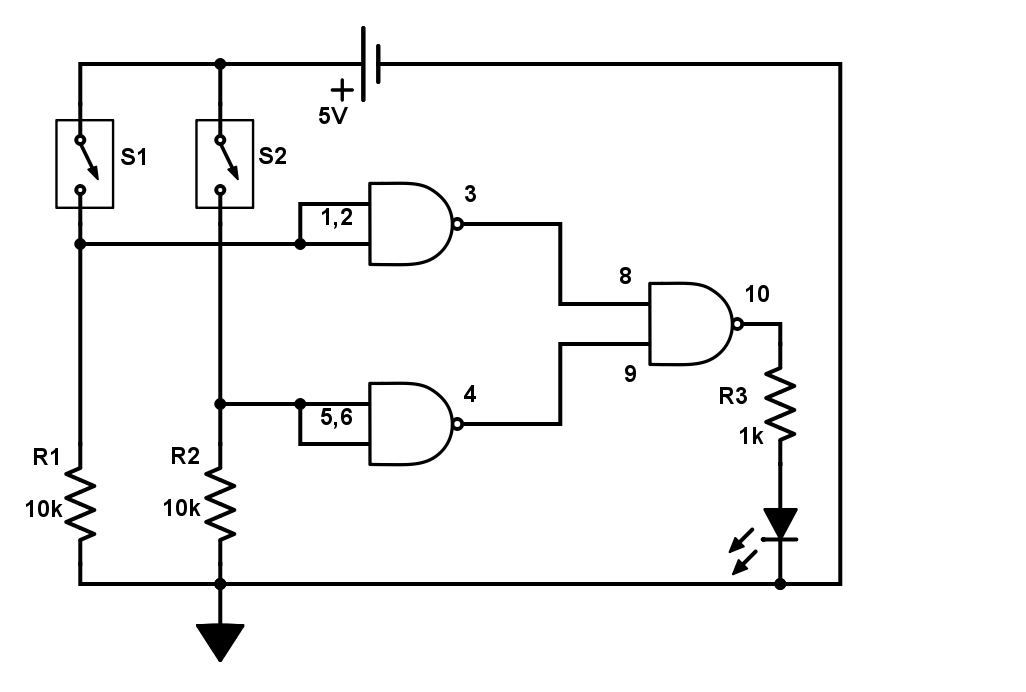
\includegraphics[scale=0.25]{NAND.png}  
    \caption{Three combined NAND gates that yields an OR gate.}
\end{figure}


Resistors can be used to restrict the current supplied to the NAND gates. The supply voltage in the circuit shown in figure (1) was 5V, so 10k$\Omega$ resistors would result in a 0.5mA current.

A 555 times is a device which produces timing pulses. A 555 timer can be used to light LEDs alternately; the schematic for this is shown in figure (2). The frequency of these pulses depend on the resistor values, $R_a$ and $R_b$, and capacitor value, $C$.

\begin{equation}
f = \frac{1.4}{C(R_a + 2R_b)}
\end{equation}

\begin{figure}[h]
    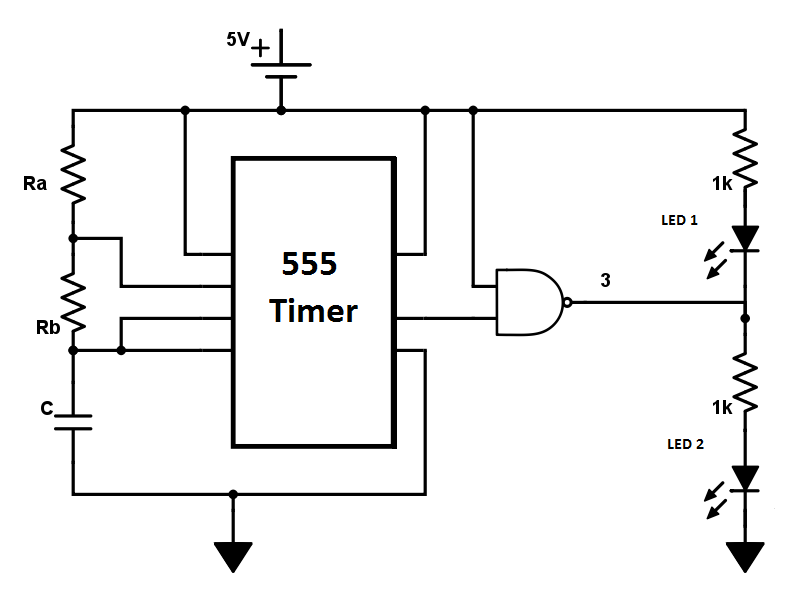
\includegraphics[scale=0.35]{555.png}  
    \caption{The alternating LED circuit built for the lab.}
\end{figure}

This circuit results in alternating lights because of the 555 timer's input to the NAND gate. The other input in is always high, because it is connected directly to the source. The input from the 555 timer alternates between high and low. When the 555 timer is high, both inputs to the NAND gate are high, and the output is low. As a result, the voltage across the first diode is 5V, and the voltage across the second diode is 0V. When the 555 timer is low, the output of the NAND gate will be high, so the voltage across the first diode will be 0V and the voltage across the second diode will be 5 V.

\section{Methodology}

%CHECK FIGURE #'s HERE
\begin{enumerate}
    \item Construct the circuit up as shown in figure (1). 
    \item Use the switches to change the input coming in and check that the output is as expected.
    \item Select/calculate values of R$_1$, R$_2$, and C such that the output of the 555 timer will be 2 Hz.
    \item Build the circuit as shown in figure (2).
    \item Test the output of the 555 timer and make sure that it is as expected.
    \item Record the output frequency of the 555 timer.
\end{enumerate}


\section{Results and Analysis}

\subsection{Data}
For for the first part of the lab, the visual feedback of the LED's was recorded. The logic table shown below illustrates the lows and highs at various points in the circuit:

\begin{center}
	\begin{ruledtabular}
    \begin{tabular}{ l l l l l l l}
	S1 & S2 & 1,2 & 5,6 & 3,8 & 4,9 & 10, LED \\ \colrule
	0 & 0 & 0 & 0 & 0 & 0 & 0  \\
	0 & 1 & 0 & 1 & 1 & 0 & 1 \\
	1 & 0 & 1 & 0 & 0 & 1 & 1  \\
	1 & 1 & 1 & 1 & 0 & 0 & 1 \\
\end{tabular}
    \end{ruledtabular}
\end{center}

For the second part of the lab, the resistor and capacitor values used in the 555 timer circuit affected the frequency of the output. The values of the resistors and capacitors used were:

\noindent $R_a = 677 k\Omega$

\noindent $R_b = 35.18 k\Omega$

\noindent $C = 0.947 \mu F$

The output frequency recorded from the output of the 555 timer was:

f$_{out}$ = 1.992 Hz


\subsection{Calculations}

Using equation (1), the expected frequency of the 555 timer was:

\begin{equation*}\label{eq:pareto mle2}
\begin{aligned}
f_{expected} &= \frac{1.4}{C(R_a + 2R_b)}\\ &= \frac{1.4}{0.947\times 10^{-6}(2(677\times 10^3) + 35.18\times 10^3}\\ &= 1.98 Hz
\end{aligned}
\end{equation*}

\noindent Using this expected frequency, the percent error could be calculated.

\begin{equation*}\label{eq:pareto mle2}
\begin{aligned}
error &= \frac{f_{out} - f_{expected}}{f_{expected}}\times100 = \frac{1.992 - 1.98}{1.98}\times100 \\ &= 0.704\%
\end{aligned}
\end{equation*}


\subsection{Analysis}

The NAND gates operated as expected in the first circuit built. The behavior of the circuit was explained in the background. Since the circuit was digital, the output does not have error, only correct or incorrect output.

For part B of the lab, the only data collected was the output frequency of the 555 timer. The output frequency only varied from the expected frequency by 0.704\%. Because the percent error was very low, it means the measurements were done accurately and the circuit was built correctly.


\section{Conclusion}

The goal of the first part of the lab was completed successfully. The desired output was obtained and checked during the lab.

For the second part of the lab, the only goal was to obtain a frequency of about 2 Hz. This was achieved with low percent error. This part of the lab was also successfully completed.

\end{document}

